\questionheader{Question 3: Dataset Preparation and Graph Construction}

\begin{itemize}
    \item \textbf{(a) Data:} The 716 San Diego sensors form one block in the LargeST metadata, adjacency and flow files, so one slice selects them everywhere (2020--2021, 210,528 five-minute steps). The values are vehicle counts, so three 5-minute values are \textbf{summed} into one 15-minute value (70,176 steps); a window with any missing value stays missing. 5.1\% of values are missing, 19 sensors never report, and the missing rate rises from about 3\% to 6\% from October 2020. A mask marks real readings so that the loss, normalisation and metrics skip filled values; gaps are forward filled (past values only), the first steps backward filled, and the 19 empty sensors set to 0. All sensors show a clear daily cycle and quieter weekends (Figure 2, left); the two directions of SR78 peak at opposite ends of the day.
    \item \textbf{(b) Graph:} 716 nodes and 17,319 weighted edges (self-loops excluded). The graph is \textbf{not symmetric}: 3,711 edges (21\%) have no reverse edge, because road distance is measured in the driving direction. A nonzero entry means sensor $j$ is a short drive from sensor $i$; weights run from 0.01 to 1 and grow as the distance shrinks. Sensors have 0 to 70 neighbours (median 20; 8 have none; Figure 3). The heatmap (Figure 2, right) shows chains of consecutive sensors along each freeway and links between the two directions and at interchanges.
\end{itemize}

\begin{center}
{\footnotesize\textbf{Figure 2: one week of 15-minute flow for three sensors (left) and the San Diego road-distance adjacency (right)}}\\[2pt]
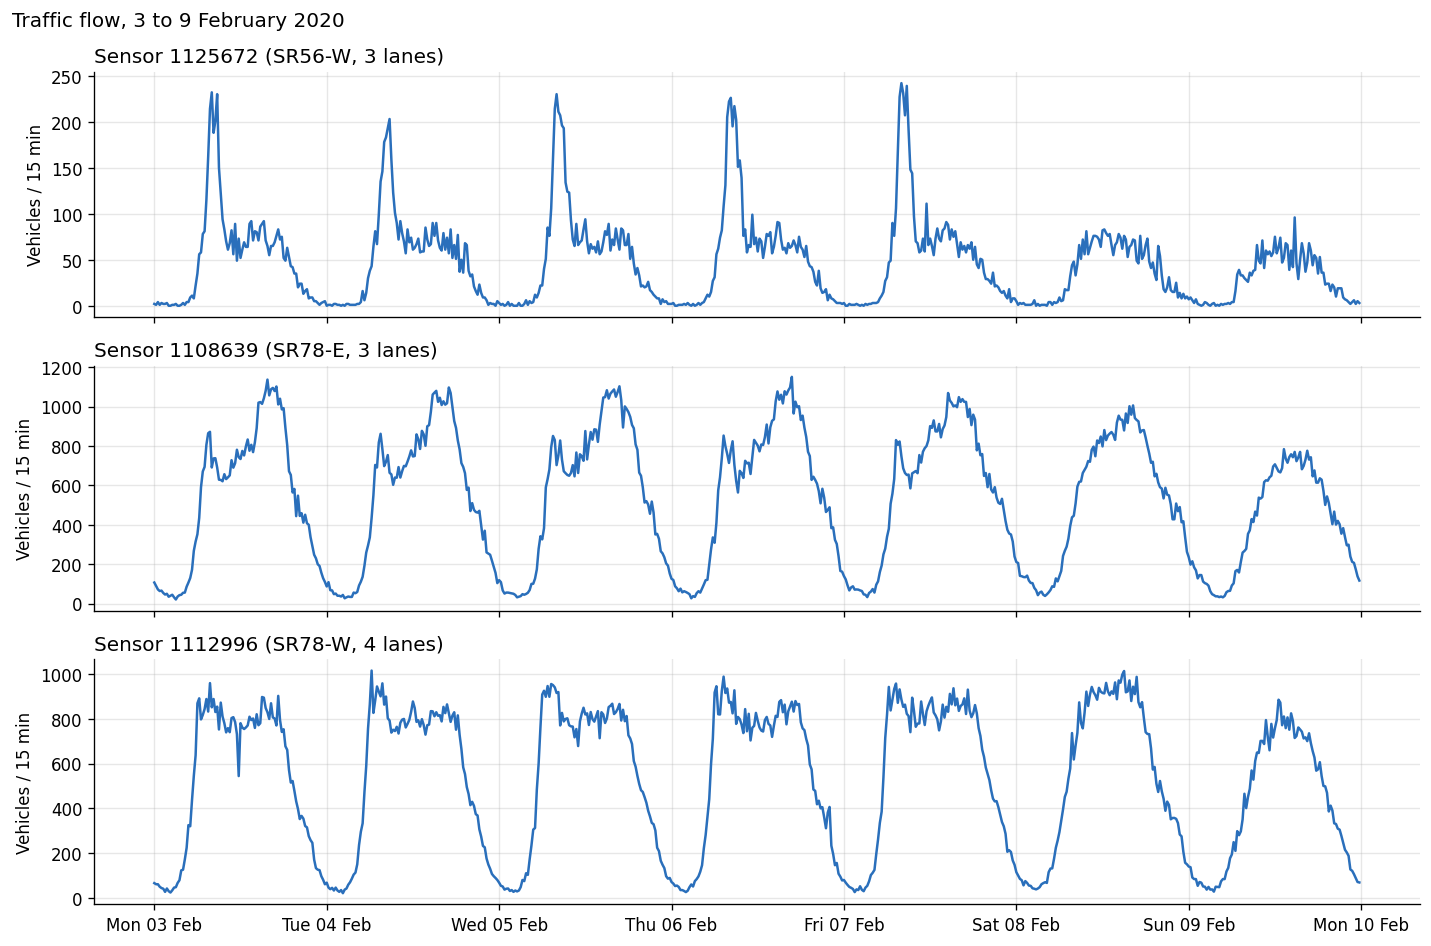
\includegraphics[height=5.2cm]{figures/q3_week.png}\hspace{10pt}%
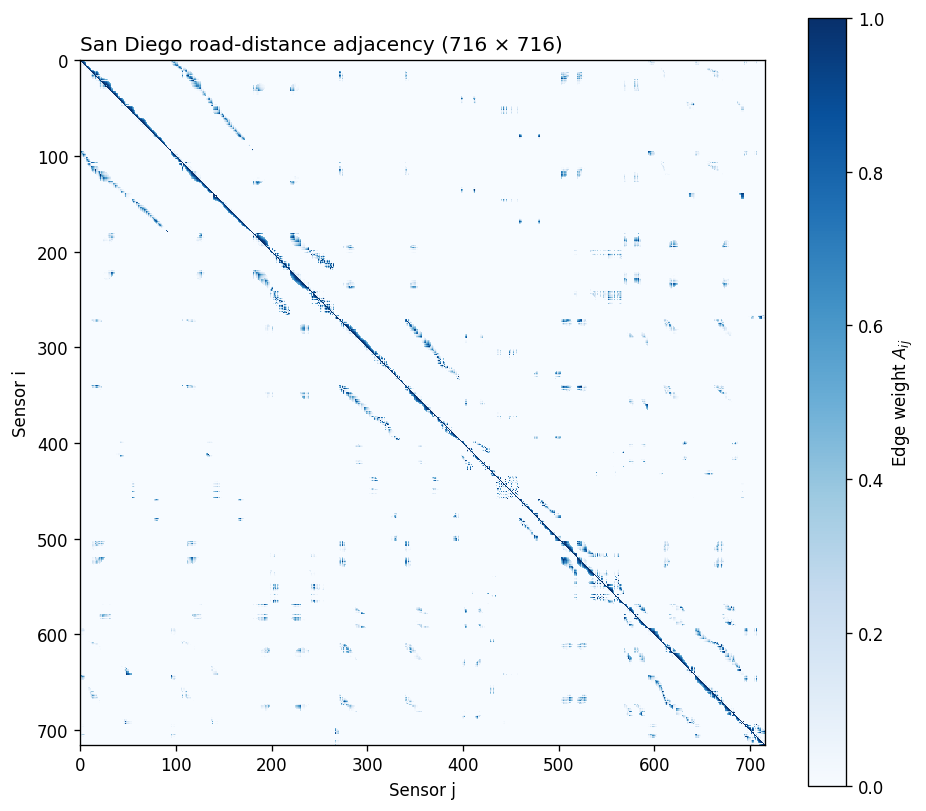
\includegraphics[height=5.2cm]{figures/q3_adjacency.png}
\end{center}

\noindent
\begin{minipage}[t]{0.56\textwidth}
\vspace{0pt}
\begin{itemize}
    \item \textbf{(c) Neighbourhoods:} Sensor 1108639 (SR78-E) has 8 one-hop neighbours and 28 within two hops; the second hop adds 13 sensors on I-5. Neighbours help because upstream traffic arrives minutes later, downstream congestion backs up, nearby sensors share demand, and they cover the sensor's own gaps; but 5 of its 8 neighbours are on the opposite direction, which peaks at a different time. One layer mixes direct neighbours; a second layer reaches neighbours of neighbours, with weaker signals. Too many layers make nearby sensors' features almost identical (over-smoothing) and squeeze many distant sensors into one vector.
\end{itemize}
\end{minipage}
\hfill
\begin{minipage}[t]{0.42\textwidth}
\vspace{2pt}
{\footnotesize\textbf{Figure 3: number of neighbours per sensor}}\\[2pt]
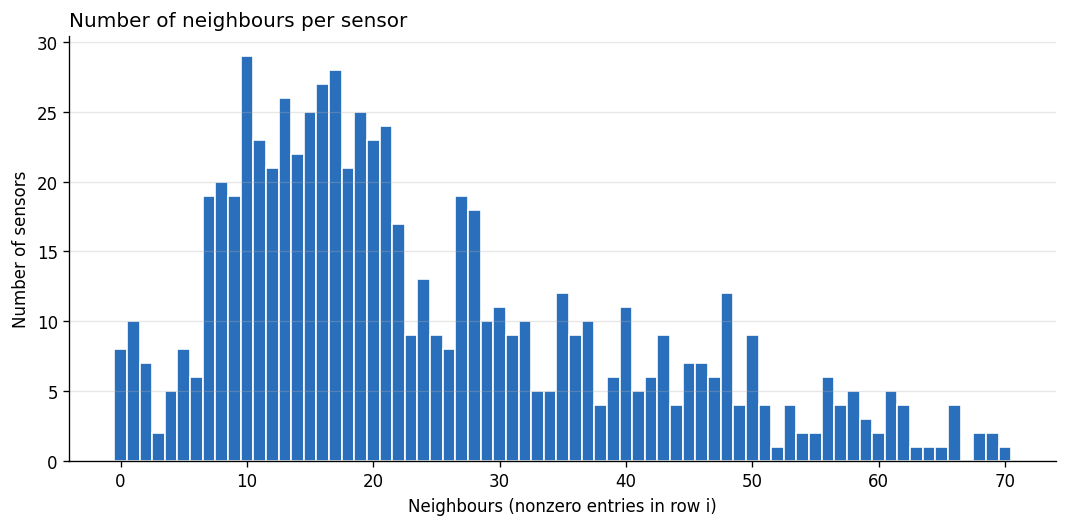
\includegraphics[width=\textwidth]{figures/q3_neighbours.png}
\end{minipage}
\vspace{4pt}
